\documentclass[12pt]{article}
\usepackage{graphicx}
\usepackage{amsmath,amssymb}
\usepackage{booktabs}
\usepackage{multirow}
\usepackage{array}
\usepackage{makecell}
\usepackage{siunitx}
\usepackage{algorithm}
\usepackage{algpseudocode}
\usepackage{hyperref}
\usepackage{setspace}

\usepackage[a4paper,margin=1in]{geometry}

% Supplementary figure/table numbering
\renewcommand{\thefigure}{S\arabic{figure}}
\renewcommand{\thetable}{S\arabic{table}}
\renewcommand{\theequation}{S\arabic{equation}}

\title{\textbf{Supplementary Information}\\
for\\
\textit{An Asynchronous Neuromorphic Architecture for Wearable EEG Emotion Recognition}}

\author{
Jingxin Liu$^{1,\dagger}$,
Yiming Zhang$^{2,\dagger}$,
Zikai Song$^{1}$,\\
Zixuan Lai$^{2}$,
Junyi Liu$^{1}$,
Fuze Tian$^{3}$,
Koo Hyoung Lee$^{4}$,\\
Qunxi Dong$^{1,*}$,
Lixian Zhu$^{1,*}$,
Bin Hu$^{1,*}$
}

\date{}

\begin{document}

\onehalfspacing

\maketitle

\begin{center}

$^{1}$Key Laboratory of Brain Health Intelligent Evaluation and Intervention (Ministry of Education),\\
School of Medical Technology, Beijing Institute of Technology, Beijing 100081, China

\vspace{4pt}

$^{2}$Key Laboratory of Brain Health Intelligent Evaluation and Intervention (Ministry of Education),\\
Beijing Institute of Technology, Zhuhai 519088, China

\vspace{4pt}

$^{3}$School of Information Science and Engineering, Lanzhou University, Lanzhou 730000, China

\vspace{4pt}

$^{4}$NeuroSky, Inc., San Jose, CA 95112, USA


\vspace{8pt}

$\dagger$ These authors contributed equally to this work.

\vspace{4pt}

$^{*}$ Corresponding authors: {dongqx}@bit.edu.cn
{zhulx}@bit.edu.cn
{bh}@bit.edu.cn
\vspace{4pt}

This work was supported by the National Natural Science Foundation of China (No. 62227807).

\end{center}

\newpage

\tableofcontents

\newpage

%--------------------------------
\section{Supplementary Methods}\label{sec:supp_methods}

\subsection{Dataset Description}\label{supp:dataset}

To evaluate the framework against prior studies, we tested it on five standard EEG datasets for emotion recognition: SEED \cite{ref65}, SEED-IV \cite{ref48}, SEED-V \cite{ref49}, DEAP \cite{ref50}, and DREAMER \cite{ref51}.

The SEED series from the BCMI laboratory at Shanghai Jiao Tong University allows performance assessment under different label granularities. We used the 62-channel EEG recordings collected during emotion elicitation via film clips. The SEED dataset includes 15 subjects across three sessions and assigns three labels: positive, neutral, and negative. SEED-IV follows an identical protocol of 15 subjects and three sessions but uses four labels (happy, sad, fear, and neutral) across 24 trials per session. SEED-V scales the experiment to 20 subjects and three sessions with 15 trials per session, using five labels: happy, sad, fear, disgust, and neutral.

The DEAP dataset comprises 32 subjects who watched 40 emotion-eliciting music videos. Ratings were reported using the Self-Assessment Manikin on a scale from 1 to 9. The EEG signals were recorded across 32 channels at 512~Hz and subsequently downsampled to 128~Hz. The DREAMER dataset includes 23 subjects and records 14 channels of EEG at 128~Hz via a wearable device. Subjects watched 18 video clips and provided ratings on a scale from 1 to 5. For both datasets, we defined a four-class classification task by combining high and low valence with high and low arousal. Continuous ratings were discretized using a threshold at the midpoint of the rating scale.

\subsection{EEG Data Preprocessing}\label{supp:preprocessing}
\begin{table}[h]
\centering
\caption{Dataset-specific preprocessing parameters. All outer windows are non-overlapping. PSE, power spectral entropy.}
\label{tab:preprocessing_params}
\vspace{2pt}
\footnotesize
\setlength{\tabcolsep}{3.5pt}
\begin{tabular}{@{}lccccc@{}}
\toprule
Dataset &
\makecell{Map size\\($H \times W$)} &
\makecell{PSE bins\\($N_f$)} &
\makecell{Outer window\\(s)} &
\makecell{Stride\\(s)} &
\makecell{PSE-bin length\\(s)} \\
\midrule
SEED      & $8 \times 9$ & 4 & 4.0 & 4.0 & 1.0 \\
SEED-IV   & $8 \times 9$ & 4 & 4.0 & 4.0 & 1.0 \\
SEED-V    & $8 \times 9$ & 4 & 4.0 & 4.0 & 1.0 \\
DEAP      & $6 \times 7$ & 6 & 9.0 & 9.0 & 1.5 \\
DREAMER   & $4 \times 5$ & 9 & 9.0 & 9.0 & 1.0 \\
\bottomrule
\end{tabular}
\end{table}

We preprocessed the EEG recordings using z-score normalization, outer windows without overlap, power spectral entropy (PSE) extraction \cite{PSE}, spatial mapping, and linear dynamical system (LDS) smoothing \cite{ref65}. Table~\ref{tab:preprocessing_params} distinguishes the duration and stride of the outer windows from the temporal bin length used to calculate PSE.

Each EEG channel was first z-score normalized. The SEED family recordings were segmented into 4-s outer windows with a 4-s stride. Four contiguous 1-s PSE bins represented each window. DEAP used 9-s outer windows with a 9-s stride and six contiguous 1.5-s PSE bins. DREAMER used 9-s outer windows with a 9-s stride and nine contiguous 1-s PSE bins. Thus, the 1-s and 1.5-s quantities specify PSE temporal bins, whereas the outer window stride is 4 or 9~s.

For spatial mapping, the PSE values from the EEG electrodes were projected onto an $H \times W$ grid according to the electrode montage, with empty grid locations set to zero. Stacking the $N_f$ temporally contiguous PSE maps yielded one tensor per outer window in $\mathbb{R}^{N_f \times H \times W}$.

Each outer window retained its \texttt{subject\_id}, \texttt{session\_id}, and \texttt{trial\_id}. For SEED, SEED-IV, and SEED-V, \texttt{session\_id} ranged from 1 to 3 and \texttt{trial\_id} denoted the trial ordinal within a session. DEAP and DREAMER were treated as single-session datasets with \texttt{session\_id}=0, and \texttt{trial\_id} denoted the trial ordinal within a subject. A trial was therefore identified by the composite key $(\texttt{subject\_id},\texttt{session\_id},\texttt{trial\_id})$.

After PSE extraction and spatial mapping, the ordered outer windows from each trial formed a sequence $\mathbf{X}^{(q)} \in \mathbb{R}^{M \times N_f \times H \times W}$. Here, $M$ is the number of outer windows in trial $q$. LDS smoothing was applied within each trial to the length-$M$ sequence at every fixed frequency--spatial coordinate $(f,h,w)$. Smoothing was confined by trial, session, and subject boundaries, and a trial with one outer window remained unchanged. LDS was applied to the complete trial sequence before creating the reported data splits. In the subject-dependent random window-level split, windows from one trial can enter both the training and held-out partitions after sharing a smoothing sequence. The subject-independent protocols exclude every window from each held-out subject during training and gradient based parameter updates.

\textbf{Complete data transformation pipeline.}
The preprocessing and inference chain can be summarized as
\begin{equation}
\underbrace{\mathbb{R}^{N_{\mathrm{ch}} \times f_s \times T_{\mathrm{trial}}}}_{\text{Raw EEG}}
\;\xrightarrow{\text{z-score and outer windows}}\;
\underbrace{\mathbb{R}^{M \times N_f \times N_{\mathrm{ch}}}}_{\text{PSE sequence within a trial}}
\;\xrightarrow{\text{Spatial map}}\;
\underbrace{\mathbb{R}^{M \times N_f \times H \times W}}_{\text{Topographic sequence}}
\;\xrightarrow{\text{LDS within each trial}}\;
\underbrace{\mathbb{R}^{M \times N_f \times H \times W}}_{\text{Smoothed sequence}}.
\label{eq:preprocessing_pipeline}
\end{equation}
Each smoothed tensor from an outer window is then processed by the depthwise separable gating module (DSGM). Division-free time-to-first-spike (DF-TTFS) encodes the features into sparse spike times, and the adaptive temporal spiking neural network (ATSNN) performs classification. These components form the dynamic adaptive spiking neural network (DA-SNN).

\textbf{Composite DSGM tensor dimensions and broadcasting.}
To specify the implementation shapes, a batch of smoothed outer window tensors is denoted by $X_0\in\mathbb{R}^{B\times N_f\times H\times W}$. Here, $B$ is the batch size, $N_f$ is the number of temporally contiguous PSE maps, and $H\times W$ is the electrode topographic grid. EEG electrodes occupy spatial grid locations, whereas $N_f$ indexes the PSE maps. The symbols below match the DSGM formulation in the main text and specify the implemented dimensions and broadcasting rules.

The depthwise separable feature transformation uses a $3\times3$ depthwise convolution with stride 2, padding 1, and $N_f$ groups. A subsequent $1\times1$ pointwise convolution maps $N_f$ input channels to $C_o=2N_f$ output channels. Its output is
\begin{equation}
U\in\mathbb{R}^{B\times C_o\times H'\times W'},\qquad
H'=\left\lfloor\frac{H+2p-k}{s}\right\rfloor+1=\left\lceil\frac{H}{2}\right\rceil,\quad
W'=\left\lceil\frac{W}{2}\right\rceil,
\label{eq:dsgm_aligned_feature}
\end{equation}
for $k=3$, $s=2$, and $p=1$. Thus, the labels showing half spatial size in Main Fig.~2 indicate stride 2 downsampling schematically. The exact integer dimensions follow Eq.~\ref{eq:dsgm_aligned_feature}, including when $H$ or $W$ is odd.

\textit{Dimensions and broadcasting by operation.}
\begin{center}
{\footnotesize
\setlength{\tabcolsep}{3pt}
\renewcommand{\arraystretch}{1.18}
\resizebox{\textwidth}{!}{%
\begin{tabular}{@{}lllllllll@{}}
\toprule
Stage/branch & Operation & Kernel & Stride & Padding & Groups & Input shape & Output shape & Broadcast at fusion \\
\midrule
Feature transform & depthwise convolution & $3\times3$ & 2 & 1 & $N_f$ & $B\times N_f\times H\times W$ & $B\times N_f\times H'\times W'$ &  \\
Feature transform & pointwise convolution & $1\times1$ & 1 & 0 & 1 & $B\times N_f\times H'\times W'$ & $B\times C_o\times H'\times W'$ &  \\
Main feature path & depthwise convolution & $3\times3$ & 1 & 1 & $C_o$ & $B\times C_o\times H'\times W'$ & $B\times C_o\times H'\times W'$ &  \\
Channel gate & global average pooling, convolution, Hard-Sigmoid & global, $1\times1$ & 1 & 0 & 1 & $B\times C_o\times H'\times W'$ & $B\times C_o\times1\times1$ & $H',W'$ axes \\
Spatial gate & channel mean, convolution, Hard-Sigmoid & $3\times3$ & 1 & 1 & 1 & $B\times C_o\times H'\times W'$ & $B\times1\times H'\times W'$ & $C_o$ axis \\
Fusion/output & Hadamard product, batch normalization, ReLU &  &  &  &  & three aligned tensors & $B\times C_o\times H'\times W'$ & PyTorch-compatible \\
\bottomrule
\end{tabular}%
}
}
\end{center}

The channel gate is broadcast across the two spatial axes, whereas the spatial gate is broadcast across the feature channel axis. The main feature tensor and both gates therefore have compatible shapes for elementwise multiplication. Batch normalization and ReLU preserve the fused tensor dimensions.

\textit{Implementation dimensions by dataset.}
\begin{center}
{\footnotesize
\setlength{\tabcolsep}{6pt}
\renewcommand{\arraystretch}{1.15}
\resizebox{\textwidth}{!}{%
\begin{tabular}{@{}lccc@{}}
\toprule
Dataset & $X_0$ without batch axis & DSGM feature/output & Flattened ATSNN input \\
\midrule
SEED / SEED-IV / SEED-V & $4\times8\times9$ & $8\times4\times5$ & 160 \\
DEAP & $6\times6\times7$ & $12\times3\times4$ & 144 \\
DREAMER & $9\times4\times5$ & $18\times2\times3$ & 108 \\
\bottomrule
\end{tabular}%
}
}
\end{center}

DF-TTFS preserves the DSGM tensor shape while mapping each dense activation to a spike time. The encoded tensor is then flattened to 160, 144, or 108 inputs for the SEED family, DEAP, or DREAMER configuration, respectively. The ATSNN classifier contains 64 and 32 hidden neurons followed by the output layer for each dataset.

\subsection{Controlled EEG Perturbation Protocol}\label{supp:controlled_perturbations}

We evaluated sensitivity to synthetic corruption on SEED, DEAP, and DREAMER. Perturbations were applied to normalized and segmented time domain EEG samples after signal conditioning for each dataset. PSE extraction, spatial mapping, and LDS smoothing followed the perturbation stage, so all downstream features were recomputed from the altered signals. The generator used a sampling rate of 200~Hz for SEED and 128~Hz for DEAP and DREAMER.

For each dataset, channel $c$, and recording unit, the standard deviation $\sigma_c$ of the clean signal was estimated over the available time domain samples. The relative noise level was defined as
\begin{equation}
\mathrm{NL}=\frac{\sigma_{n,c}}{\sigma_c},
\label{eq:relative_noise_level}
\end{equation}
where $\sigma_{n,c}$ is the standard deviation of the generated perturbation after normalization within each channel. We evaluated $\mathrm{NL}\in\{0.01,0.03,0.05,0.08,0.10,0.125\}$ together with the unperturbed condition (Clean, NL$=0$).

Three perturbation families were generated. Gaussian corruption consisted of independent white noise with zero mean, scaled to $\mathrm{NL}\,\sigma_c$. Low frequency drift was produced by a first order Butterworth low pass filter applied to a white noise trace spanning the session. The filter used a 0.5-Hz cutoff, and the resulting trace was normalized within each channel before scaling to the target NL. Electromyographic (EMG)-like corruption consisted of transient bursts triggered by a Poisson process along the recording time axis. The generator used an average event rate of 0.5 bursts per second per channel and Gaussian envelopes with full width at half maximum sampled uniformly from 20 to 50~ms. Carrier frequencies and conversions from seconds to samples followed the sampling rate of each dataset. Each carrier band remained below the corresponding Nyquist frequency. Each EMG-like trace was normalized by its root mean square within each channel and then scaled to $\mathrm{NL}\,\sigma_c$.

For reproducibility, a deterministic noise seed was derived for each dataset recording, perturbation type, and NL. Within each condition, DA-SNN, DH-SNN, and EEGNet used the same generated feature bundle, random window-level 80/20 split, model seed, training schedule, checkpoint selection rule, and evaluation level. Every perturbation type and NL used a separate training and model selection run matched to that noise condition. The reported trajectories use one model seed and are summarized by individual accuracies and descriptive differences between Clean and NL$=0.125$. Error bars and significance tests require repeated model seeds and are outside this analysis.

\subsection{Implementation Details}
Experiments were conducted on a computing server equipped with a 12-core Intel\textsuperscript{\textregistered} Xeon\textsuperscript{\textregistered} Platinum 8255C CPU at 2.50~GHz and an NVIDIA GeForce RTX 2080 Ti GPU with 11~GB of memory. The software environment consisted of Ubuntu 22.04, Python 3.12, PyTorch 2.3.0, and CUDA 12.1.

For conventional machine learning baselines, hyperparameters followed the cited implementations. For deep learning models, we used the AdamW optimizer \cite{ref64} to minimize cross entropy loss with a learning rate of $1\times10^{-4}$ and a batch size of $8$. Training proceeded for a maximum of $200$ epochs with early stopping. Performance was evaluated using window-level accuracy (Acc), macro-F1 (F1), and macro-specificity (Spe).

Table~\ref{tab:training_config} summarizes the complete training configuration.

\begin{table}[h]
\centering
\caption{Training configuration.}
\label{tab:training_config}
\footnotesize
\renewcommand{\arraystretch}{1.2}
\setlength{\tabcolsep}{4pt}
\begin{tabular}{@{}ll@{}}
\toprule
Parameter & Value \\
\midrule
Optimizer & AdamW \\
Learning rate & $1 \times 10^{-4}$ \\
Learning-rate schedule & CosineAnnealingLR, $\eta_{\min} = 1 \times 10^{-6}$ \\
Batch size & 8 \\
Max epochs & 200 \\
Early stopping patience & 30 \\
Early stopping min\_delta & $1 \times 10^{-4}$ \\
Weight initialization & Xavier uniform \\
Loss function & Cross-entropy \\
Random seeds & 1, 2, 3, 4, 5 \\
Hardware & NVIDIA RTX 2080 Ti \\
Framework & PyTorch 2.3.0, CUDA 12.1 \\
\bottomrule
\end{tabular}
\end{table}

To assess deployment on constrained platforms, we performed inference experiments on a Raspberry Pi~5 with a quad-core 64-bit BCM2712 processor (ARM Cortex-A76 architecture). The device runs Linux and executes an 8-bit integer (INT8) model.

We also implemented this INT8 model on a Xilinx Zynq-7000 system-on-chip (SoC) with an XC7Z020 device (speed grade -2, CLG400 package). This implementation evaluates field-programmable gate array (FPGA) deployment on programmable logic. We analyzed the implemented resource utilization, including lookup tables (LUTs), flip-flops (FFs), block RAMs (BRAMs), and digital signal processing slices (DSPs), to quantify the on-chip hardware footprint.

\subsection{Evaluation Protocols, Model Selection, and Statistics}\label{supp:evaluation_protocols}

Table~\ref{tab:eval_protocol} consolidates the dataset composition, temporal construction, and the two evaluation objectives used in this study. Main Table~1 reports a subject-dependent benchmark under a random window-level 80/20 split for all five datasets. Complementary subject-independent evaluations use leave-one-subject-out (LOSO) or fixed subject-holdout splits and are reported in Supplementary Tables~\ref{tab:cross_subject_seed} and \ref{tab:cross_subject_deap_dreamer}.

\begin{table}[h]
\centering
\caption{Dataset composition and evaluation protocols. The ``4/4/1'', ``9/9/1.5'', and ``9/9/1'' entries denote outer-window duration/stride/PSE-bin length in seconds.}
\label{tab:eval_protocol}
\scriptsize
\renewcommand{\arraystretch}{1.25}
\setlength{\tabcolsep}{3pt}
\resizebox{\textwidth}{!}{%
\begin{tabular}{@{}lcccccc@{}}
\toprule
Dataset & Subjects & Sessions & Trials & \makecell{Outer window/stride/\\PSE bin (s)} & Main benchmark & Subject-independent evaluation \\
\midrule
SEED    & 15 & 3 & 15/session & 4/4/1 & Random windows, 80/20 & LOSO, 15 held-out-subject splits \\
SEED-IV & 15 & 3 & 24/session & 4/4/1 & Random windows, 80/20 & LOSO, 15 held-out-subject splits \\
SEED-V  & 20 & 3 & 15/session & 4/4/1 & Random windows, 80/20 & LOSO, 20 held-out-subject splits \\
DEAP    & 32 & 1 & 40/subject & 9/9/1.5 & Random windows, 80/20 & Five fixed splits, 26 train/6 held-out subjects \\
DREAMER & 23 & 1 & 18/subject & 9/9/1 & Random windows, 80/20 & Five fixed splits, 19 train/4 held-out subjects \\
\bottomrule
\end{tabular}%
}
\end{table}

\textbf{Subject-dependent main benchmark.}
For Main Table~1, the split unit was the outer window. Approximately 80\% of the pooled windows were assigned to training and 20\% to a held-out evaluation partition using random splitting stratified by class. Windows from the same subject, and potentially the same trial, can occur in both partitions. This subject-dependent protocol provides a common benchmark for the 15 models. Its scope is comparison among overlapping subjects and trials, whereas unseen subject generalization is evaluated separately below.

\textbf{Subject-independent supplementary evaluations.}
For SEED, SEED-IV, and SEED-V, leave-one-subject-out (LOSO) evaluation held out one complete subject per split. All sessions, trials, and windows from that subject were excluded during training and gradient based parameter updates. For DEAP and DREAMER, we used five predefined subject holdout splits across subjects. Each DEAP split contained 26 training subjects and 6 held-out subjects. Each DREAMER split contained 19 training subjects and 4 held-out subjects. These fixed holdouts use an approximately 80/20 subject ratio and differ from both within-subject splitting and mutually exclusive fivefold cross-validation.

\textbf{Checkpoint selection.}
The reported EEG protocols used no separate validation subset. For each predefined split, accuracy on the held-out evaluation partition was measured after every epoch for checkpoint selection and early stopping. The selected checkpoint was then used to calculate the reported metrics on the same partition. Neural models in the unified reevaluation followed the same split definitions and checkpoint selection rule. In subject-independent evaluations, every sample from a held-out subject remained excluded during training and gradient based parameter updates. Model selection and final reporting use the same held-out partition, so the resulting estimates represent comparisons within each protocol rather than performance on an untouched independent test set.

\textbf{Metrics and aggregation.}
Accuracy is the proportion of correctly classified held-out windows. Macro-F1 is the unweighted mean of the F1 scores for each class. Macro-specificity treats each class in a one-versus-rest manner. For each class, specificity is calculated as $\mathrm{TN}/(\mathrm{TN}+\mathrm{FP})$ from true negatives (TN) and false positives (FP), followed by an unweighted mean across classes. When measurements for repeats or splits were available, we report the arithmetic mean and sample standard deviation (\texttt{ddof}=1). Main Table~1 reports DA-SNN as mean $\pm$ sample standard deviation across repeated runs, while baseline point estimates are retained as available. The SEED family LOSO results are reported as mean $\pm$ sample standard deviation across splits of held-out subjects. The DEAP and DREAMER records contain aggregate point estimates over the five predefined subject holdout splits. Dispersion values were unavailable for these records and are omitted.
%--------------------------------
\section{Supplementary Notes}

\subsection{B1 Model Definition and Forward Semantics}

ATSNN adopts the B1 model introduced by Stanojevi\'{c} et~al. \cite{ref46} as its spike time substrate. In their general formulation, the identity mapping uses $A_i^{(n)}=0$ and $B_i^{(n)}=1$ for every neuron $i$ and layer $n$. The latter fixes the threshold crossing slope to unity. Each hidden neuron emits at most one spike in the half-open layer window $[T_{\min}^{(n)},T_{\max}^{(n)})$. Adjacent windows satisfy the cascade condition $T_{\min}^{(n)}=T_{\max}^{(n-1)}$. We assume $\epsilon>0$, $T_{\max}^{(n)}>T_{\min}^{(n)}$, and parameters that place the theoretical crossing of an active neuron within its assigned window. Here, $\vartheta_i^{(n)}$ is the firing threshold in normalized membrane potential units, and $\epsilon\vartheta_i^{(n)}$ is its temporal offset.

Solving the dynamics with constant slope gives the theoretical first passage time
\begin{equation}
\tilde{T}_i^{(n)} = T_{\min}^{(n)} + \epsilon\vartheta_i^{(n)} + \sum_j W_{ij}^{(n)}\!\left(T_j^{(n-1)} - T_{\min}^{(n)}\right).
\label{eq:supp_theoretical_time}
\end{equation}
This crossing becomes an active spike only if it occurs strictly before the upper boundary:
\begin{equation}
M_i^{(n)} = \mathbf{1}\!\left[\tilde{T}_i^{(n)} < T_{\max}^{(n)}\right].
\label{eq:b1_mask}
\end{equation}
The observed, censored time is
\begin{equation}
T_i^{(n)} = M_i^{(n)}\tilde{T}_i^{(n)} + \bigl(1-M_i^{(n)}\bigr)T_{\max}^{(n)}.
\label{eq:supp_actual_time}
\end{equation}
Thus, $M_i^{(n)}=1$ denotes an active neuron, whereas $M_i^{(n)}=0$ denotes an inactive neuron whose stored time is the boundary placeholder. Equality at $T_{\max}^{(n)}$ is assigned to the inactive case. The mask is used when identifying valid events and updating temporal windows. In the forward map, the cascade condition also makes the inactive placeholder equal to the next layer's reference time, so its temporal offset is exactly zero.

For the original B1 identity parameterization, the derivative of the theoretical crossing time with respect to its weighted temporal input $I_i^{(n)}$ is constant,
\begin{equation}
\frac{\partial \tilde{T}_i^{(n)}}{\partial I_i^{(n)}}=1,
\qquad
I_i^{(n)}=\sum_j W_{ij}^{(n)}\!\left(T_j^{(n-1)}-T_{\min}^{(n)}\right),
\label{eq:b1_slope}
\end{equation}
and the latency $\tau_i^{(n)}=T_{\max}^{(n)}-T_i^{(n)}$ can be mapped to a ReLU activation under the weight, threshold, and window assumptions of Ref.~\cite{ref46}:
\begin{equation}
\tau_i^{(n)}=\mathrm{ReLU}\!\left(\sum_j W_{ij}^{(n)}\tau_j^{(n-1)}+b_i^{(n)}\right).
\label{eq:b1_relu}
\end{equation}
This correspondence motivates the selection of B1 as a tractable substrate for hardware.

The original B1 work also adapts $T_{\max}$ during training through a conditional rule centered on the upper boundary. ATSNN builds on this established concept with the signed error rule in Eq.~(\ref{eq:supp_window_update}), referenced to the window midpoint. The rule contracts or expands the window according to the earliest valid spike. DA-SNN integrates this regulation with DSGM processing for EEG, power-of-two DF-TTFS encoding, and the globally asynchronous, locally synchronous (GALS) accelerator.

\subsection{Division-Free TTFS Encoding Derivation}

TTFS coding maps higher activation values to earlier spike times, generating at most one spike per neuron within a given inference cycle. Standard TTFS encoding normalizes input activations using floating-point division:
\begin{equation}
V_{\mathrm{norm}} = \frac{V_{\mathrm{in}}-V_{\min}}{V_{\max}-V_{\min}},
\end{equation}
where $V_{\mathrm{in}}$ is the input activation, and $V_{\min}$ and $V_{\max}$ denote the activation bounds. Because floating-point division introduces computational overhead, the proposed division-free encoder replaces it with power-of-two scaling. 

During training, the activation range $(V_{\max}-V_{\min})$ is monitored to define a scaling factor $S_p$ as the smallest power of two bounding this range:
\begin{equation}
S_p = 2^{\lceil \log_2(\max(V_{\max}-V_{\min},\,\delta)) \rceil},
\end{equation}
where $\delta=10^{-5}$ in the float32 training implementation. The exponent $\lceil\log_2(\cdot)\rceil$ is retained as an integer shift count, so $S_p$ is implemented by a power-of-two shift in fixed-point inference. If $V_{\max}=V_{\min}$, the safeguard keeps $S_p$ positive; all normalized activations are then zero and map to the boundary code $T_{\mathrm{spike}}=T_{\max}$ rather than causing division by zero.

After training, parameters $V_{\min}$ and $S_p$ are fixed to ensure deterministic encoding during inference. The normalized activation then becomes
\begin{equation}
V_{\mathrm{norm}} = \mathrm{clip}\left(\frac{V_{\mathrm{in}}-V_{\min}}{S_p},0,1\right),
\end{equation}
where $\mathrm{clip}(\cdot)$ constrains the value to the interval $[0,1]$. This normalized value is mapped to a spike time within the temporal window:
\begin{equation}
T_{\mathrm{spike}} = T_{\max}-\mathrm{round}\left(V_{\mathrm{norm}}(T_{\max}-T_{\min})\right).
\end{equation}

This formulation preserves the TTFS ordering in which stronger activations correspond to earlier spike times. At the hardware level, a threshold filter discards candidates outside the assigned temporal window and serializes the remaining valid events into address-event representation (AER) packets.

\subsection{Local Weight Gradient Relation and Adaptive Temporal Window Regulation}

\textbf{Forward map convention.}
The analysis below uses the theoretical crossing time, active mask, and censored observed time defined in Eqs.~(\ref{eq:supp_theoretical_time})--(\ref{eq:supp_actual_time}). An active neuron has $M_i^{(n)}=1$ and $T_i^{(n)}=\tilde{T}_i^{(n)}$; an inactive neuron has $M_i^{(n)}=0$ and stores the boundary placeholder $T_{\max}^{(n)}$.

\textbf{Proposition 1 (Weight gradient).}
For neuron $i$ in layer $n$, the gradient of the loss function $\mathcal{L}$ with respect to synaptic weight $W_{ij}^{(n)}$ is given by the chain rule:
\begin{equation}
\frac{\partial \mathcal{L}}{\partial W_{ij}^{(n)}} =
\frac{\partial \mathcal{L}}{\partial T_i^{(n)}}
\cdot
\frac{\partial T_i^{(n)}}{\partial W_{ij}^{(n)}}.
\label{eq:supp_chain_rule}
\end{equation}

For active neurons ($T_i^{(n)}=\tilde{T}_i^{(n)}$), differentiating Eq.~(\ref{eq:supp_theoretical_time}) yields
\[
\frac{\partial T_i^{(n)}}{\partial W_{ij}^{(n)}} =
T_j^{(n-1)} - T_{\min}^{(n)}.
\]

For silent neurons, $T_i^{(n)}$ is constant at $T_{\max}^{(n)}$, rendering the gradient zero almost everywhere. Thus, the weight gradient follows the piecewise form

\begin{equation}
\frac{\partial \mathcal{L}}{\partial W_{ij}^{(n)}} =
\begin{cases}
\displaystyle
\frac{\partial \mathcal{L}}{\partial T_i^{(n)}}
\left(
T_j^{(n-1)} - T_{\min}^{(n)}
\right),
& \tilde{T}_i^{(n)} < T_{\max}^{(n)} \\[1.0ex]
0,
& \tilde{T}_i^{(n)} \ge T_{\max}^{(n)}.
\end{cases}
\label{eq:supp_gradient_piecewise}
\end{equation}

\textbf{Definition 1 (Temporal offset).}
The presynaptic temporal offset is defined as
\[
\Delta T_{ij}^{(n)} = T_j^{(n-1)} - T_{\min}^{(n)}.
\]

For active neurons, the gradient magnitude is

\[
\left|
\frac{\partial \mathcal{L}}{\partial W_{ij}^{(n)}}
\right|
=
\left|
\frac{\partial \mathcal{L}}{\partial T_i^{(n)}}
\right|
\cdot
|\Delta T_{ij}^{(n)}|.
\]

\textbf{Adaptive window regulation.}
Let the valid-spike set be $\mathcal{V}^{(n)}=\{T_i^{(n)}\mid M_i^{(n)}=1\}$. When $\mathcal{V}^{(n)}\neq\emptyset$, its earliest valid spike is
\[
T_e^{(n)}=\min \mathcal{V}^{(n)}.
\]
The window update rule is

\begin{equation}
T_{\max}^{(n)\prime} =
T_{\max}^{(n)}
+
\lambda
\left(
T_e^{(n)} -
\frac{T_{\max}^{(n)}+T_{\min}^{(n)}}{2}
\right).
\label{eq:supp_window_update}
\end{equation}
If $\mathcal{V}^{(n)}=\emptyset$, no $T_e^{(n)}$ is formed and the fallback is $T_{\max}^{(n)\prime}=T_{\max}^{(n)}$. After an update, a minimum width $\delta_T=10^{-4}$ is enforced so that $T_{\max}^{(n)\prime}\ge T_{\min}^{(n)}+\delta_T$. This mechanism contracts the window when valid spikes occur before the midpoint and expands it when they occur after the midpoint.

The complete procedure of this mechanism is detailed in Algorithm~\ref{alg:atsnn_update}.

\begin{algorithm}[H]
\caption{Forward pass and adaptive temporal window update.}
\label{alg:atsnn_update}
\begin{algorithmic}[1]
\Require $T^{(n-1)},W^{(n)},\vartheta^{(n)},\epsilon,\lambda,T_{\min}^{(n)},T_{\max}^{(n)},\delta_T,\mathrm{mode}$
\Ensure $T^{(n)},M^{(n)},T_{\max}^{(n)\prime}$
\State $T_{\min}^{(n)}\gets T_{\max}^{(n-1)}$ \Comment{Cascade boundary}
\State $T_{\max}^{(n)\prime}\gets T_{\max}^{(n)}$ \Comment{Default and empty-set fallback}
    \Statex \textit{Phase 1: Censored B1 model forward pass}
\For{each neuron $i$ in layer $n$}
    \State $S_i\gets\sum_j W_{ij}^{(n)}\bigl(T_j^{(n-1)}-T_{\min}^{(n)}\bigr)$
    \State $\tilde{T}_i^{(n)}\gets T_{\min}^{(n)}+\epsilon\vartheta_i^{(n)}+S_i$
    \State $M_i^{(n)}\gets\mathbf{1}[\tilde{T}_i^{(n)}<T_{\max}^{(n)}]$
    \State $T_i^{(n)}\gets M_i^{(n)}\tilde{T}_i^{(n)}+(1-M_i^{(n)})T_{\max}^{(n)}$
\EndFor
    \Statex \textit{Phase 2: Window update referenced to the midpoint}
\If{$\mathrm{mode}=\texttt{train}$}
    \State $\mathcal{V}^{(n)}\gets\{T_i^{(n)}\mid M_i^{(n)}=1\}$
    \If{$\mathcal{V}^{(n)}\neq\emptyset$}
        \State $T_e^{(n)}\gets\min\mathcal{V}^{(n)}$
        \State $\bar{T}_{\max}\gets T_{\max}^{(n)}+\lambda\left(T_e^{(n)}-(T_{\max}^{(n)}+T_{\min}^{(n)})/2\right)$
        \State $T_{\max}^{(n)\prime}\gets\max\bigl(\bar{T}_{\max},T_{\min}^{(n)}+\delta_T\bigr)$
    \EndIf
\EndIf
\State $T_{\min}^{(n+1)}\gets T_{\max}^{(n)\prime}$
\State \Return $T^{(n)},M^{(n)},T_{\max}^{(n)\prime}$
\end{algorithmic}
\end{algorithm}

\textbf{Continuous output readout and inactive neuron semantics.}
The final layer is nonspiking and integrates the latency coded hidden representation into real valued class logits. Because $T_{\min}^{(L)}=T_{\max}^{(L-1)}$, an inactive hidden neuron stores $T_j^{(L-1)}=T_{\max}^{(L-1)}=T_{\min}^{(L)}$ and contributes exactly zero. Therefore, the implemented readout from observed times is algebraically identical to an explicitly masked readout:
\begin{equation}
\begin{aligned}
z_k
&=\sum_j W_{kj}^{(L)}\!\left(T_{\min}^{(L)}-T_j^{(L-1)}\right)+\epsilon\vartheta_k^{(L)}\\
&=\sum_j W_{kj}^{(L)}M_j^{(L-1)}\!\left(T_{\min}^{(L)}-\tilde{T}_j^{(L-1)}\right)+\epsilon\vartheta_k^{(L)}.
\end{aligned}
\label{eq:masked_logit}
\end{equation}
The explicit mask identifies the scalar boundary placeholder as inactive. It is used to determine event validity, adapt the window, and distinguish active from censored neurons in subsequent analyses.

\subsection{Quantization Strategy}
We represent the model with signed INT8 weights and unsigned 8-bit nonnegative activations, allowing inference with integer arithmetic. This choice reduces the data volume of weights and activations and suits FPGA execution. Uniform 8-bit quantization assigns a separate scale to each weight or activation tensor. We use symmetric scaling for weights and an offset of zero for nonnegative activations. For a real valued weight tensor $r$, the scale $s_w$ and signed quantizer $Q_s(\cdot)$ are
\begin{equation}
\begin{aligned}
s_w &= \frac{\max\!\left(\max(|r|),\epsilon_q\right)}{127},\\
Q_s(r) &= \mathrm{clip}\!\left(\mathrm{round}\!\left(\frac{r}{s_w}\right),-127,127\right),
\qquad \hat{r}=s_w Q_s(r),
\end{aligned},
\label{eq:quant_w}
\end{equation}

where $\epsilon_q>0$ keeps the denominator positive for a tensor containing only zeros. The factor 127 maps the positive and negative extrema to $+127$ and $-127$, respectively, with symmetric clipping. The additional INT8 code $-128$ remains unused.

For a nonnegative activation tensor $r$, the unsigned scale $s_a$ and quantizer $Q_u(\cdot)$ are
\begin{equation}
\begin{aligned}
s_a &= \frac{\max\!\left(\max(r),\epsilon_q\right)}{255},\\
Q_u(r) &= \mathrm{clip}\!\left(\mathrm{round}\!\left(\frac{r}{s_a}\right),0,255\right),
\qquad \hat{r}=s_a Q_u(r),
\end{aligned},
\label{eq:quant_a}
\end{equation}
where the activation maximum used to determine $s_a$ is obtained from the complete SEED training partition in the random window-level 80/20 protocol. Calibration uses only the training partition, and the resulting scale for each activation tensor is fixed during inference. Both quantizers round to the nearest integer and then saturate values to the stated ranges.

We apply quantization-aware training to mitigate accuracy loss during quantization. Starting from the converged floating-point model, training resumes with a smaller learning rate while $Q_s(\cdot)$ and $Q_u(\cdot)$ are applied in the forward pass. After each update, weights are projected back onto the quantized set \cite{ref26}. Batch Normalization (BN) folding is performed offline by merging each BN transformation into the weights and biases of the preceding convolution before integer inference.



\subsection{Detailed Hardware Control Protocol}
The accelerator follows a globally asynchronous, locally synchronous (GALS) organization with two independent local clock islands. The input and feature buffers, tensor compute engine (TCE), multibranch fusion path, and division-free TTFS encoder operate in the \texttt{clk\_TCE} island. The weight memory, compute unit and processing element (CU/PE) arrays, spike collector, and final layer state operate in the \texttt{clk\_SNN} island. A downstream comparator tree consumes the final 32-bit membrane potentials. Each island retains its own execution clock. The AER block forms a composite boundary. The sending side forms packets and generates requests (Req), clock domain crossing (CDC) synchronization occurs at the boundary, and the \texttt{clk\_SNN} side handles routing, broadcasting, and hidden layer recirculation.

Event transfer uses a bundled-data four-phase protocol. When DF-TTFS generates a valid spike time $t_i$, the sending interface places the address and timestamp on the payload bus, allows the bus to stabilize, and asserts Req. The payload remains unchanged throughout the Req--Ack transaction. Req passes through a synchronizer with two stages into the \texttt{clk\_SNN} island. The receiver then samples the stable payload and decodes its destination from the current layer and controller state. It enables the required CU/PE array and schedules the membrane potential update. When all target updates for the event are complete, the receiver asserts acknowledgment (Ack). Ack returns through a synchronizer with two stages to the \texttt{clk\_TCE} island.

\begin{figure}[h]
\centering
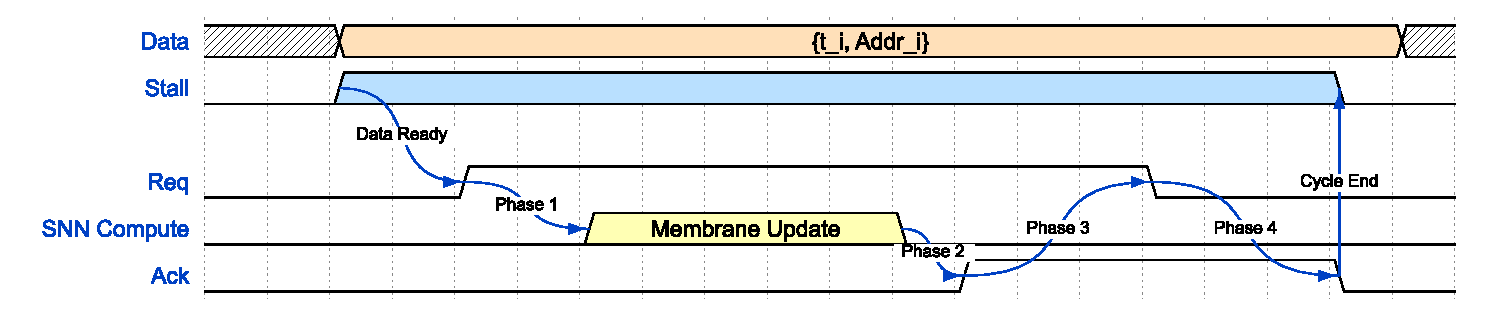
\includegraphics[width=\columnwidth]{figures/timingdiagram.eps} 
\caption{Timing diagram of the bundled-data four-phase handshake between the locally synchronous \texttt{clk\_TCE} and \texttt{clk\_SNN} islands. The address/timestamp payload is stabilized before request (Req) assertion and held until the synchronized acknowledgment (Ack) completes the transfer.}
\label{fig:handshake_timing}
\end{figure}

As illustrated in Fig.~\ref{fig:handshake_timing}, the transfer proceeds through four control transitions. The sender asserts Req after stabilizing the payload. The receiver observes synchronized Req and asserts Ack after processing the event. The sender then observes synchronized Ack and deasserts Req, followed by Ack at the receiver after synchronized Req becomes low. The sender releases or replaces the payload only after synchronized Ack returns low. The bundled-data stability rule maintains the multibit address and timestamp bus while synchronized single bit controls define the sampling and release window.

The stall behavior provides backpressure by holding the sender while a transfer remains outstanding. The AER/CDC path implements this control directly through the handshake. The only first-in, first-out (FIFO) buffer shown in Main Fig.~4(b) belongs to the TCE line buffer. Thus, the handshake protects the bundled payload during transfer.

The implementation uses register clock enables controlled by local finite state machines. A dedicated clock gating primitive such as BUFGCE is outside the confirmed implementation. In the \texttt{clk\_TCE} island, the controller schedules the main, channel gating, and spatial gating paths. It clears the clock enable of a completed path while waiting for the remaining paths. In the \texttt{clk\_SNN} island, layer and array enables select compute resources for reuse over time. Inactive registers and datapaths retain state with their local clock enables deasserted.

The single GALS Flow Controller coordinates start, enable, completion, and layer or array state. Idle is a local finite state after completion, and the Req/Ack stall behavior supplies backpressure. The controller carries only control and status signals. Tensor and spike payloads remain on their data paths, and each island retains its local execution clock.

\subsubsection*{GALS boundary and clock domain considerations.}
Both compute regions are locally synchronous. The \texttt{clk\_TCE} signal updates TCE state, and \texttt{clk\_SNN} updates SNN state. Two stage synchronizers receive the single bit Req and Ack controls in their respective domains. The payload instead follows the bundled-data stability rule. This structure reduces CDC metastability risk. Quantitative mean time between failures requires device parameters and a timing report beyond the present analysis.

\subsubsection*{Sources of energy efficiency.}
The architecture has three distinct efficiency mechanisms. First, \emph{event sparsity in the model}: TTFS generates at most one spike per neuron per inference cycle. Censored neurons generate no event, reducing AER transfers, weight reads, and membrane updates. Second, \emph{event-triggered execution and data movement}: routing, local memory access, and CU/PE updates occur only for accepted events. Third, \emph{local clock enable control}: completed or inactive datapaths retain state and avoid unnecessary clocked updates. The third mechanism reduces dynamic switching activity while leaving static power unchanged. The matched synchronous comparison below evaluates the net implementation trade-off, including mechanisms beyond event rate alone.

\subsubsection*{GALS interface overhead.}
The GALS interface consumes logic and adds transfer latency. It includes valid event filtering, AER routing and broadcasting, hidden layer recirculation, address decoding, two stage synchronizers in both directions, four-phase handshake state machines, and clock enable control. Each accepted event therefore incurs routing and protocol work even in a sparse stream. Top level hierarchical synthesis resolves the LUT and flip-flop counts and functional latencies reported below. Dynamic power remains aggregated for the complete accelerator, so the analysis assigns no separate power percentage to an interface component.

\subsection{Streaming Line Buffer for Convolution}
To sustain convolution throughput under streaming input conditions, the tensor compute engine uses a shift register line buffer to reconstruct sliding convolution windows on the chip \cite{conv}.

The line buffer acts as a cascade of FIFO registers storing recent input samples from the data stream. When a new EEG sample enters the pipeline, the buffer updates its internal state via column shifting. This process reconstructs the spatial context required for convolution without repeatedly accessing external memory. For a $3\times3$ convolution kernel, the buffer maintains three rows of feature data, continuously forming local windows by combining the current input with stored samples. The resulting sliding window is forwarded to the multiply-accumulate pipeline every clock cycle.

This reconstruction converts a serialized data stream into parallel convolution windows while avoiding repeated external memory reads for each local window. During multibranch execution, concurrent access from the main branch, channel gate, and spatial gate exceeds the limit of two ports in standard BRAMs. The architecture therefore implements a multibank buffer with one write stream and three read streams per pipeline stage. BRAM replication and scheduled reads provide the required access pattern for each branch. Throughput remains subject to the stated pipeline and interface timing.

\begin{figure}[htbp]
  \centering
  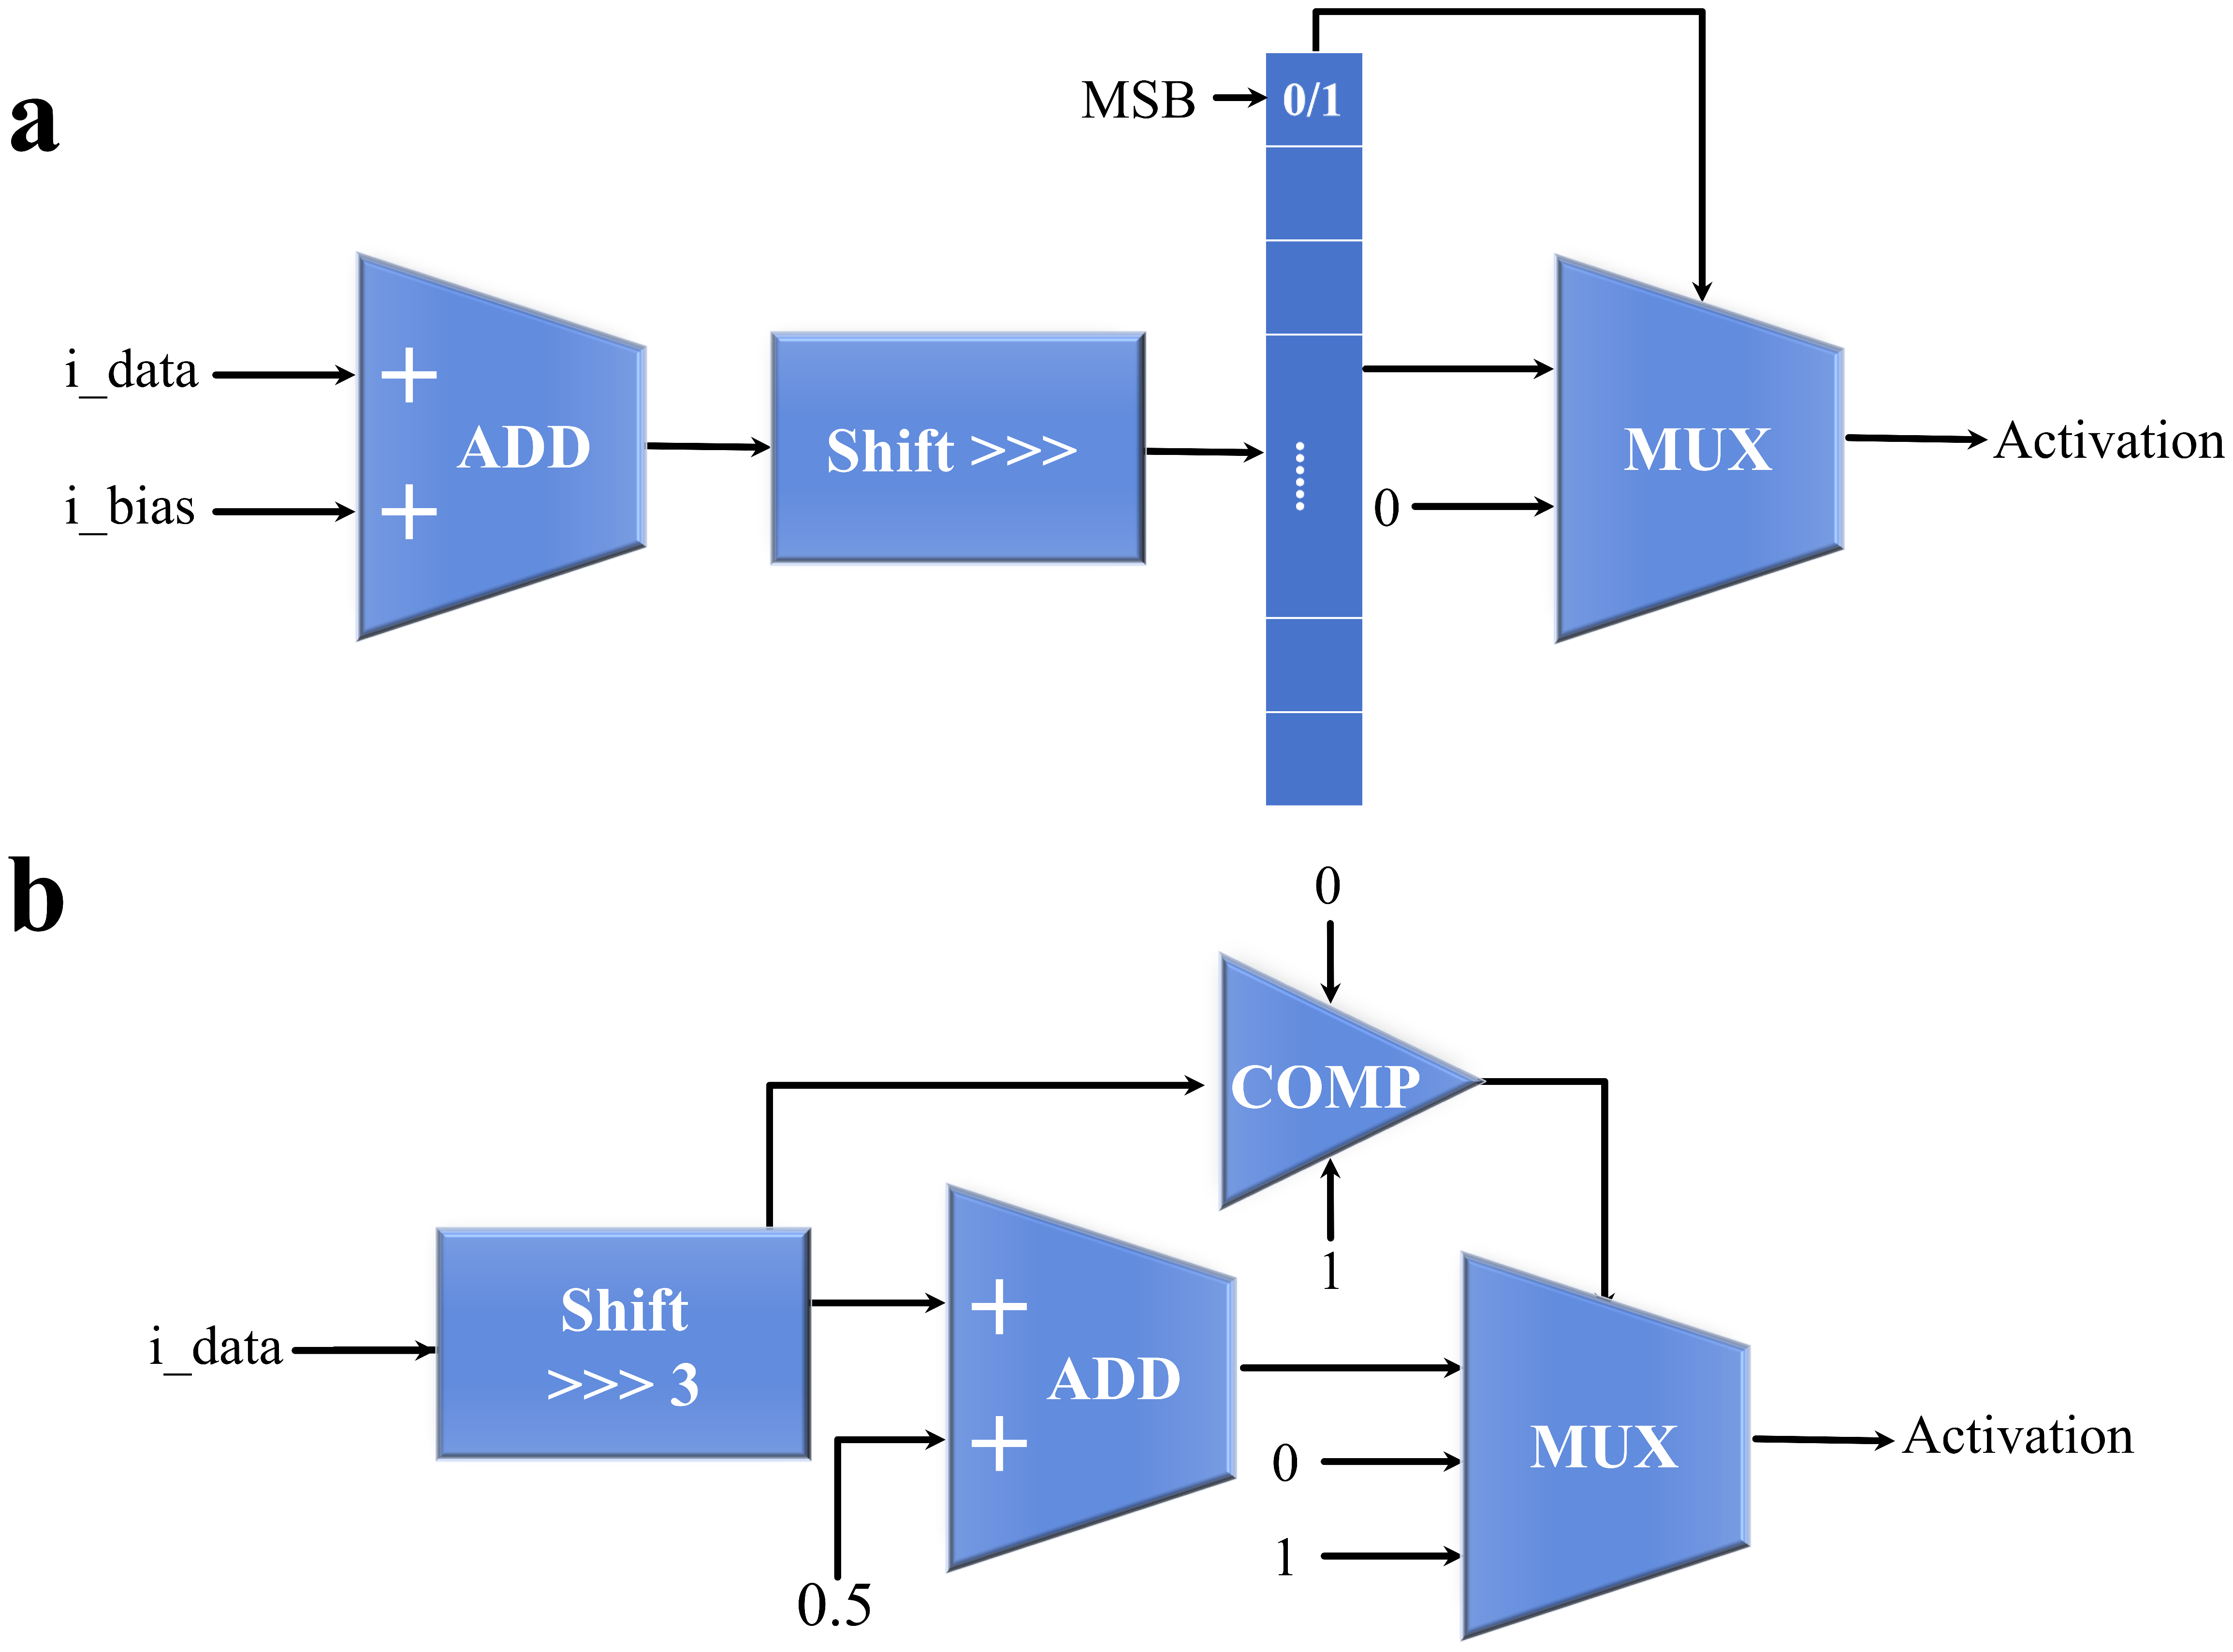
\includegraphics[width=0.8\columnwidth]{figures/BNRELUHSigmoid.eps}
  \caption{\textbf{Hardware architecture of batch normalization and Hard-Sigmoid modules.}
  (a) Batch normalization datapath with parameter folding and quantization. 
  (b) Hard-Sigmoid implementation using shift, add, and clamp operations.}
  \label{fig:BN_RELU_HSigmoid}
\end{figure}

\subsection{Hardware Realization of Batch Normalization and Hard-Sigmoid}
To reduce pipeline depth, the output stage integrates logic that performs batch normalization, quantization, and activation within a single datapath. As shown in Fig.~\ref{fig:BN_RELU_HSigmoid}(a), we use the linearity of convolution to apply an offline parameter folding strategy, merging normalization parameters into the preceding convolution weights and biases. For the Hard-Sigmoid function in the gating paths, we implement a circuit using shift, add, and clamp operations (Fig.~\ref{fig:BN_RELU_HSigmoid}(b)) to avoid exponential calculations. The input is shifted right by three bits and biased by a fixed-point constant (0.5), followed by clamping via comparators.

\subsection{Event-Driven Processing Element Microarchitecture}
Each SNN processing element (PE) follows an event-driven execution model controlled by a local finite-state machine (FSM) in the \texttt{clk\_SNN} island. The FSM schedules accepted events and uses a register clock enable to hold inactive state during idle periods.

By default, the PE is idle and its state-update clock enable is deasserted. When the synchronized AER request is accepted and the array is selected, the FSM asserts the enable and activates the datapath. During computation, the PE performs a time-modulated multiply-accumulate operation. The datapath subtracts a local reference time from the incoming spike timestamp to obtain the temporal difference. This difference is multiplied by the synaptic weight and accumulated into a 32-bit membrane-potential register.

After computation, the PE asserts a local completion status and enters a wait state. The array barrier aggregates completion from the active PEs, and the AER receiver asserts Ack after the event update is complete. The PE then returns to idle and deasserts its clock enable. This mechanism avoids unnecessary state updates when no valid event is being processed. The local clock network continues to operate.


\subsection{Memory Centered SNN Array Organization}

To address frequent weight access in spiking neural networks, the compute fabric places weight storage beside computation. Each SNN array integrates a dedicated static random access memory (SRAM) interface that supplies one 32-bit word per read cycle. The word is unpacked into four INT8 weights and routed to four processing elements, providing four weights per memory read.

Multiple SNN arrays operate in parallel and connect via the AER interface, which broadcasts incoming spike events across the fabric. For hidden layers, internally generated spike events recirculate through the same interface to support time-multiplexed execution of subsequent layers on the same physical hardware.

Upon reaching the final layer, results stream to the decision unit. A combinational comparator tree identifies the index of the maximum 32-bit membrane potential. The result is read in the same cycle without an additional pipeline stage.

\subsection{Barrier Synchronization Mechanism}

Each locally synchronous array integrates a lightweight barrier synchronizer to coordinate parallel execution while retaining its local clock.

The synchronizer uses a counter to track completion signals from active processing elements within the array. When a PE finishes computing the current event, it increments the counter. The synchronizer asserts an array completion signal when the count matches the number of active neurons scheduled for the current layer. This barrier completes all partial membrane updates before the next event and prevents races between concurrent computations. The mechanism operates locally within each array, while completion remains a control signal rather than a clock.
%--------------------------------
\section{Supplementary Experiments}

\subsection{Subject-Independent Generalization Across EEG Benchmarks}\label{supp:cross_subject}

We additionally evaluated generalization to unseen subjects using LOSO for the SEED family datasets and five fixed subject holdout splits for DEAP and DREAMER. These protocols use different split units and statistical aggregation from the subject-dependent benchmark in Main Table~1. Their absolute values therefore describe a separate evaluation setting. Among the 10 models in each subject-independent setting, DA-SNN ranked first in accuracy, macro-F1, and macro-specificity across all five datasets.

\begin{table}[!htbp]
\centering
\caption{Subject-independent leave-one-subject-out (LOSO) performance on the SEED-family datasets. Values are mean $\pm$ sample standard deviation across held-out-subject splits (\%). Acc, window-level accuracy; F1, macro-F1; Spe, macro-specificity. Best results are shown in bold.}
\label{tab:cross_subject_seed}
\scriptsize
\renewcommand{\arraystretch}{1.18}
\setlength{\tabcolsep}{2.4pt}
\resizebox{\textwidth}{!}{%
\begin{tabular}{@{}lccccccccc@{}}
\toprule
\multirow{2}{*}{Method} & \multicolumn{3}{c}{SEED} & \multicolumn{3}{c}{SEED-IV} & \multicolumn{3}{c}{SEED-V} \\
\cmidrule(lr){2-4}\cmidrule(lr){5-7}\cmidrule(lr){8-10}
& Acc & F1 & Spe & Acc & F1 & Spe & Acc & F1 & Spe \\
\midrule
ShuffleNetV2       & $58.43\pm9.66$ & $56.86\pm10.26$ & $79.25\pm4.81$ & $51.25\pm4.12$ & $48.20\pm4.60$ & $78.71\pm1.37$ & $42.96\pm5.42$ & $38.81\pm4.63$ & $83.30\pm1.26$ \\
Deep ConvNet       & $58.27\pm10.65$ & $54.72\pm12.59$ & $79.14\pm5.36$ & $51.24\pm5.34$ & $46.83\pm7.67$ & $79.13\pm1.89$ & $47.00\pm5.87$ & $39.66\pm8.03$ & $83.14\pm1.66$ \\
MobileNetV3-Small  & $57.08\pm8.48$ & $55.15\pm9.53$ & $78.57\pm4.23$ & $51.23\pm4.16$ & $48.43\pm5.31$ & $78.73\pm1.36$ & $47.36\pm6.13$ & $43.54\pm6.69$ & $83.66\pm1.47$ \\
EEGNet             & $56.69\pm11.00$ & $54.88\pm11.79$ & $78.37\pm5.46$ & $53.82\pm5.52$ & $50.76\pm6.34$ & $79.06\pm1.88$ & $43.32\pm5.17$ & $38.02\pm6.13$ & $82.94\pm1.27$ \\
MobileNetV3-Large  & $56.69\pm8.00$ & $55.34\pm8.26$ & $78.41\pm3.94$ & $50.99\pm3.96$ & $48.01\pm4.92$ & $78.66\pm1.18$ & $41.12\pm5.39$ & $37.80\pm4.97$ & $82.94\pm1.19$ \\
DH-SNN             & $56.36\pm10.03$ & $53.07\pm11.37$ & $78.17\pm5.04$ & $51.95\pm5.07$ & $47.42\pm6.75$ & $78.94\pm1.74$ & $42.29\pm6.07$ & $34.61\pm8.26$ & $82.85\pm1.72$ \\
Shallow ConvNet    & $56.27\pm9.02$ & $51.77\pm10.44$ & $78.13\pm4.55$ & $52.62\pm5.00$ & $43.47\pm6.27$ & $78.27\pm1.78$ & $43.66\pm6.23$ & $32.52\pm8.20$ & $82.47\pm1.79$ \\
EfficientNet-B0    & $55.57\pm9.68$ & $53.37\pm10.04$ & $77.81\pm4.85$ & $50.18\pm3.76$ & $46.76\pm3.89$ & $78.80\pm1.27$ & $43.93\pm4.50$ & $38.29\pm5.25$ & $82.80\pm1.10$ \\
SqueezeNet         & $36.88\pm8.95$ & $22.13\pm14.29$ & $68.34\pm4.50$ & $45.78\pm3.04$ & $29.27\pm2.52$ & $75.00\pm1.06$ & $38.81\pm4.03$ & $21.80\pm3.01$ & $80.00\pm1.07$ \\
\textbf{DA-SNN}   & $\mathbf{59.10\pm6.93}$ & $\mathbf{57.60\pm7.18}$ & $\mathbf{80.00\pm3.47}$ & $\mathbf{55.80\pm4.55}$ & $\mathbf{52.40\pm5.76}$ & $\mathbf{79.80\pm1.53}$ & $\mathbf{48.20\pm4.50}$ & $\mathbf{44.40\pm5.60}$ & $\mathbf{84.30\pm1.19}$ \\
\bottomrule
\end{tabular}%
}
\end{table}

\begin{table}[!htbp]
\centering
\caption{Cross-subject performance on DEAP and DREAMER using five fixed subject-holdout splits (\%). Acc, window-level accuracy; F1, macro-F1; Spe, macro-specificity. The available records provide aggregate point estimates across the five splits; dispersion values are therefore not reported. Best results are shown in bold.}
\label{tab:cross_subject_deap_dreamer}
\footnotesize
\renewcommand{\arraystretch}{1.18}
\setlength{\tabcolsep}{4pt}
\resizebox{\textwidth}{!}{%
\begin{tabular}{@{}lcccccc@{}}
\toprule
\multirow{2}{*}{Method} & \multicolumn{3}{c}{DEAP: 26 train/6 held-out subjects} & \multicolumn{3}{c}{DREAMER: 19 train/4 held-out subjects} \\
\cmidrule(lr){2-4}\cmidrule(lr){5-7}
& Acc & F1 & Spe & Acc & F1 & Spe \\
\midrule
MobileNetV3-Large & 52.49 & 32.27 & 75.31 & 61.81 & 38.32 & 76.26 \\
DH-SNN            & 51.26 & 32.51 & 75.63 & 60.14 & 31.51 & 75.19 \\
ShuffleNetV2      & 51.22 & 30.41 & 75.24 & 59.63 & 35.47 & 75.40 \\
Deep ConvNet      & 52.47 & 31.62 & 75.12 & 60.57 & 34.08 & 76.06 \\
Shallow ConvNet   & 52.68 & 30.68 & 75.11 & 59.90 & 31.27 & 75.33 \\
EfficientNet-B0   & 51.16 & 30.04 & 75.17 & 60.34 & 31.69 & 75.90 \\
EEGNet            & 50.94 & 31.31 & 75.13 & 58.36 & 39.16 & 76.57 \\
MobileNetV3-Small & 51.92 & 32.88 & 75.30 & 58.04 & 35.13 & 75.53 \\
SqueezeNet        & 43.90 & 24.71 & 75.00 & 61.48 & 33.33 & 75.41 \\
\textbf{DA-SNN}  & \textbf{54.30} & \textbf{35.60} & \textbf{76.30} & \textbf{64.80} & \textbf{43.40} & \textbf{77.20} \\
\bottomrule
\end{tabular}%
}
\end{table}


\subsection{Ablation Studies}

We expanded the ablation study from SEED to SEED, DEAP, and DREAMER to test the principal components across different channel configurations and emotion label structures. Five controlled conditions were evaluated under the subject-dependent random window-level 80/20 protocol. The first three were the complete DA-SNN, standard convolution in place of depthwise separable convolution, and removal of DSGM. The remaining conditions used conventional floating-point min--max normalization or fixed temporal windows for each layer. Each condition used the same five random seeds (1--5). Table~\ref{tab:supp_ablation} reports the arithmetic mean and sample standard deviation (\texttt{ddof}=1) across these five runs.

The descriptive mean differences reveal both shared effects and effects that vary by dataset. Replacing the adaptive window with fixed windows lowers mean accuracy by 4.98, 10.75, and 0.83 percentage points on SEED, DEAP, and DREAMER, respectively. Removing DSGM lowers mean accuracy by 3.20, 17.58, and 0.37 points. Replacing depthwise separable convolution lowers it by 1.87, 4.84, and 5.40 points. The smaller changes on DREAMER for DSGM and the adaptive window indicate that effect magnitude depends on the dataset. Conventional min--max normalization changes mean accuracy by $+0.06$, $-1.07$, and $+0.66$ points relative to DF-TTFS on SEED, DEAP, and DREAMER, respectively. These mixed directions place the main role of DF-TTFS in replacing floating-point division with power-of-two scaling for hardware implementation. The reported differences are descriptive means; no significance tests were performed.

\begin{table}[htbp]
\centering
\caption{Cross-dataset ablation results under the subject-dependent random window-level 80/20 protocol. Values are mean $\pm$ sample standard deviation across five random seeds (1--5). Acc, window-level accuracy; F1, macro-F1; Spe, macro-specificity.}
\label{tab:supp_ablation}
\footnotesize
\renewcommand{\arraystretch}{1.2}
\setlength{\tabcolsep}{5pt}
\resizebox{\textwidth}{!}{
\begin{tabular}{@{}llccc@{}}
\toprule
Dataset & Variant & Acc (\%) & F1 (\%) & Spe (\%) \\
\midrule
\multirow{5}{*}{SEED}
 & Full DA-SNN & $96.85 \pm 1.44$ & $96.81 \pm 0.92$ & $97.08 \pm 0.87$ \\
 & Standard convolution & $94.98 \pm 0.51$ & $94.95 \pm 1.06$ & $95.17 \pm 0.45$ \\
 & Without DSGM & $93.65 \pm 0.78$ & $93.78 \pm 1.33$ & $93.41 \pm 1.00$ \\
 & Standard min--max & $96.91 \pm 1.02$ & $96.89 \pm 1.46$ & $97.15 \pm 1.08$ \\
 & Fixed temporal window & $91.87 \pm 0.54$ & $91.82 \pm 0.68$ & $92.03 \pm 1.45$ \\
\midrule
\multirow{5}{*}{DEAP}
 & Full DA-SNN & $87.96 \pm 5.44$ & $86.83 \pm 8.53$ & $97.62 \pm 3.20$ \\
 & Standard convolution & $83.12 \pm 6.32$ & $81.89 \pm 1.79$ & $95.75 \pm 2.80$ \\
 & Without DSGM & $70.38 \pm 3.16$ & $67.27 \pm 3.95$ & $91.25 \pm 5.70$ \\
 & Standard min--max & $86.89 \pm 1.55$ & $74.93 \pm 5.48$ & $93.68 \pm 7.96$ \\
 & Fixed temporal window & $77.21 \pm 2.46$ & $75.18 \pm 5.83$ & $93.77 \pm 5.32$ \\
\midrule
\multirow{5}{*}{DREAMER}
 & Full DA-SNN & $94.18 \pm 2.20$ & $91.73 \pm 2.56$ & $94.38 \pm 4.64$ \\
 & Standard convolution & $88.78 \pm 1.42$ & $84.99 \pm 2.38$ & $92.43 \pm 4.70$ \\
 & Without DSGM & $93.81 \pm 5.01$ & $90.95 \pm 4.52$ & $94.27 \pm 0.88$ \\
 & Standard min--max & $94.84 \pm 2.92$ & $92.83 \pm 3.63$ & $96.31 \pm 2.81$ \\
 & Fixed temporal window & $93.35 \pm 1.55$ & $91.00 \pm 3.29$ & $95.33 \pm 0.78$ \\
\bottomrule
\end{tabular}
}
\end{table}

Figure~\ref{fig:supp_window_evolution} provides a behavioral diagnostic for the adaptive temporal window. In this representative SEED trajectory over 200 epochs, the first hidden layer interval evolves from $[1.00,2.00]$ to $[2.26,12.25]$. The second evolves from $[2.00,3.00]$ to $[12.25,40.42]$. Their widths increase from 1.00 to 9.98 and 28.17, respectively, before entering comparatively narrow ranges late in training. Over the final 20 epochs, the widths measured across epochs within the run are $9.91\pm0.19$ and $28.17\pm0.30$. This trajectory shows adaptation specific to each layer and settling late in training.

\begin{figure}[htbp]
\centering

\includegraphics[width=\textwidth]{figures/window_evolution.pdf}
\caption{Adaptive temporal window evolution during one representative 200-epoch training run on SEED. Solid and dashed curves denote the upper and lower boundaries of each layer, respectively, and dotted curves denote window width. Each value is recorded after the corresponding training epoch. Variations over the final 20 epochs describe temporal fluctuations within this run. Table~\ref{tab:supp_ablation} separately reports performance across random seeds when adaptive boundaries are replaced with fixed windows.}
\label{fig:supp_window_evolution}
\end{figure}

\subsection{Hardware Measurement Boundary and Standalone Preprocessing Kernels}

The reported 18~$\mu$s latency and 40/108/148~mW dynamic/static/total power describe one accelerator inference from a preprocessed input tensor to the class output. The board power measurement uses the programmable logic (PL) accelerator boundary. It includes on-chip input and feature buffers, the PL serial peripheral interface (SPI), tensor compute engine (TCE), multibranch fusion path, and DF-TTFS encoder. The boundary also includes valid event filtering, the AER/CDC interface, weight memory, CU/PE arrays, spike collector, controller, and final decision logic. EEG acquisition, PSE extraction, LDS smoothing within each trial, processing system (PS) cores, external double data rate (DDR) memory, and board peripherals lie outside this boundary. Table~\ref{tab:system_inclusion} records the included components.

\begin{table}[!htbp]
\centering
\caption{System inclusion boundary for the reported GALS accelerator latency, power, and energy. ``Included'' denotes membership in the board measurement of the accelerator. The 2.66~$\mu$J value covers these components, while separately characterized kernels are reported individually.}
\label{tab:system_inclusion}
\scriptsize
\renewcommand{\arraystretch}{1.16}
\setlength{\tabcolsep}{3pt}
\resizebox{\textwidth}{!}{%
\begin{tabular}{@{}lccc@{}}
\toprule
Stage or component & 18~$\mu$s latency & 40/108/148~mW power & 2.66~$\mu$J energy \\
\midrule
PSE extraction & Excluded; standalone kernel & Excluded & Excluded \\
Trial-wise LDS smoothing & Excluded; standalone kernel & Excluded & Excluded \\
PL input/feature buffers and SPI-side interface & Included & Included & Included \\
TCE, multi-branch fusion, and DF-TTFS & Included & Included & Included \\
Event filter, AER/CDC, handshake, and controller & Included & Included & Included \\
Weight memory, CU/PE arrays, spike collector, and readout & Included & Included & Included \\
PS cores, external DDR, EEG acquisition, and board peripherals & Excluded & Excluded & Excluded \\
\bottomrule
\end{tabular}%
}
\end{table}

PSE and LDS were implemented and measured on the same FPGA board as independent kernels. Their latency and power values are standalone measurements under the workload and boundary of each kernel. Table~\ref{tab:preprocessing_kernels} reports the PSE result for one call with 200 samples. It reports the LDS result for 864 outputs, implemented as 288 lanes over three test steps, which covers part of a trial. Each energy value is calculated from the independently measured total power and latency of the corresponding kernel. PSE, LDS, and accelerator inference were tested separately, so their static power and energy values represent separate measurements rather than an integrated system total.

\begin{table}[!htbp]
\centering
\caption{Standalone FPGA measurements of preprocessing kernels at board level. PSE, LDS, and the GALS accelerator were tested independently, and each power and energy value retains its own measurement boundary. Power components were rounded independently.}
\label{tab:preprocessing_kernels}
\scriptsize
\renewcommand{\arraystretch}{1.15}
\setlength{\tabcolsep}{2.3pt}
\resizebox{\textwidth}{!}{%
\begin{tabular}{@{}lrrrrclrrrrr@{}}
\toprule
Kernel & LUT & FF & BRAM & DSP & \makecell{Clock\\(MHz)} & Workload & \makecell{Latency\\(ms)} & \makecell{Dynamic power\\(mW)} & \makecell{Static power\\(mW)} & \makecell{Total power\\(mW)} & \makecell{Energy\\($\mu$J)} \\
\midrule
PSE & 13,550 & 479 & 34 & 44 & 2 & one 200-sample call & 10.25 & 7 & 106 & 113 & 1,158.25 \\
LDS & 4,797 & 374 & 1 & 8 & 4 & 288 lanes $\times$ 3 steps & 0.216 & 5 & 105 & 109 & 23.544 \\
\bottomrule
\end{tabular}%
}
\end{table}

\subsection{FPGA Resource Utilization and GALS Interface Cost}

We evaluated the deployment characteristics of the accelerator using the Zynq-7020 implementation. As detailed in Table~\ref{tab:fpga_resource}, the complete design occupies a limited fraction of the available programmable logic. The interface figures in Table~\ref{tab:gals_component_overhead} are components attributed by hierarchical synthesis of the complete design.

\begin{table}[!htbp]
\centering
\caption{FPGA resource utilization of the complete GALS accelerator.}
\label{tab:fpga_resource}
\footnotesize
\renewcommand{\arraystretch}{1.2}
\setlength{\tabcolsep}{4pt}
\begin{tabular}{@{}lrrr@{}}
\toprule
Resource & Used & Available & Utilization (\%) \\
\midrule
LUT & 10,822 & 53,200 & 20.34 \\
FF & 8,164 & 106,400 & 7.67 \\
BRAM & 22 & 140 & 15.71 \\
DSP & 32 & 220 & 14.55 \\
\bottomrule
\end{tabular}
\end{table}

\begin{table}[!htbp]
\centering
\caption{Hierarchical synthesis breakdown of logic associated with the GALS interface. Functional latencies describe individual blocks and are reported separately. The six component budget is the gross attributed footprint; the matched comparison in the text below reports the net resource difference.}
\label{tab:gals_component_overhead}
\scriptsize
\renewcommand{\arraystretch}{1.15}
\setlength{\tabcolsep}{3pt}
\begin{tabular}{@{}lrrl@{}}
\toprule
Component & LUT & FF & Functional latency \\
\midrule
Threshold/event-valid filter & 93 & 42 & 1 cycle \\
AER arbitration/router & 512 & 286 & 2 cycles \\
Address decoder & 148 & 79 & 1 cycle \\
Req/Ack synchronizers & 26 & 36 & 3 destination-clock cycles per crossing \\
Four-phase handshake FSM & 87 & 53 & 11 cycles per complete handshake \\
Clock-enable controller & 115 & 106 & 1 cycle \\
\midrule
Six-component budget & 981 & 602 & Not additive \\
Complete GALS accelerator & 10,822 & 8,164 & 18~$\mu$s per inference \\
\bottomrule
\end{tabular}
\end{table}

The six reported components account for 981 LUTs and 602 FFs, corresponding to 9.1\% and 7.4\% of the complete GALS design, respectively. These gross counts include logic with functional counterparts in the synchronous implementation. The matched implementation comparison below provides the net resource difference. Power is measured for the complete accelerator and is not partitioned by synthesis hierarchy.

\subsection{FPGA Deployment Comparisons}

To isolate the effect of the GALS organization in this implementation, we compared it with a synchronous version of the same INT8 DA-SNN. Both versions use the same Zynq-7020 platform and input tensor. The synchronous version replaces the Req/Ack boundary between two islands with a ready/valid interface under one clock, while retaining clock enable control. At the 100-MHz target, the synchronous design uses 10,650 LUTs, 8,025 FFs, 22 BRAMs, and 32 DSPs. It completes 1,650 cycles per inference (16.5~$\mu$s). GALS uses 10,822 LUTs, 8,164 FFs, 22 BRAMs, and 32 DSPs and completes 1,800 cycles (18~$\mu$s). The GALS and synchronous implementations achieve $F_{\max}$ values of 105.3 and 108.7~MHz, respectively. Their dynamic/static/total power values are 40/108/148 and 96/107/203~mW. These values give dynamic/total energy values of 0.72/2.66 and 1.58/3.35~$\mu$J per inference. GALS adds 172 LUTs (1.62\%) and 139 FFs (1.73\%) and increases latency by 9.09\%. It reduces measured board dynamic power by 58.3\% and total energy per inference by 20.6\%. This matched comparison establishes the net energy advantage for the present implementation; broader asynchronous designs require their own matched measurements.

To provide a hardware baseline across models, EEGNet was also deployed on the Zynq-7020. Table~\ref{tab:fpga_eegnet_comparison} reports the resource, latency, power, and energy results for both FPGA deployments. The models and clock organizations differ, so this comparison characterizes deployment trade-offs. The matched comparison above isolates the effect of GALS.

\begin{table}[!htbp]
\centering
\caption{FPGA deployment comparison of the GALS DA-SNN accelerator and EEGNet on Zynq-7020. Energy per inference is calculated from total power and inference latency. The different model architectures and clock targets define this as a deployment comparison; the preceding text provides the matched GALS comparison.}
\label{tab:fpga_eegnet_comparison}
\scriptsize
\renewcommand{\arraystretch}{1.14}
\setlength{\tabcolsep}{4pt}
\begin{tabular}{@{}lcrr@{}}
\toprule
Metric & Unit & GALS DA-SNN & EEGNet \\
\midrule
LUT & count & 10,822 & 6,977 \\
FF & count & 8,164 & 3,097 \\
BRAM & count & 22 & 6 \\
DSP & count & 32 & 5 \\
Clock target & MHz & 100 & 50 \\
Inference latency & $\mu$s & 18 & 772 \\
Dynamic power & mW & 40 & 32 \\
Static power & mW & 108 & 106 \\
Total power & mW & 148 & 138 \\
Total energy/inference & $\mu$J & 2.66 & 106.536 \\
\bottomrule
\end{tabular}
\end{table}

Compared with EEGNet, the GALS DA-SNN uses more LUTs, FFs, BRAMs, and DSPs and 7.25\% higher total power. Its inference latency is nevertheless 97.67\% lower, and its total energy per inference is 97.50\% lower. Equivalently, the EEGNet deployment requires approximately 42.9 times the latency and 40.0 times the total energy of the GALS DA-SNN deployment under their respective implementation settings.

\subsection{FPGA Latency and Energy Measurement}

Table~\ref{tab:power_comparison} summarizes the absolute GALS accelerator metrics. Total energy is calculated as $148~\mathrm{mW}\times18~\mu\mathrm{s}=2.664~\mu\mathrm{J}$ and reported as 2.66~$\mu$J. The corresponding dynamic energy is $40~\mathrm{mW}\times18~\mu\mathrm{s}=0.72~\mu\mathrm{J}$.

\begin{table}[!htbp]
\centering
\caption{GALS FPGA latency, power, and energy within the accelerator inference boundary.}
\label{tab:power_comparison}
\footnotesize
\renewcommand{\arraystretch}{1.2}
\setlength{\tabcolsep}{4pt}
\begin{tabular}{@{}lrr@{}}
\toprule
Metric & Value & Unit \\
\midrule
Latency & 18 & $\mu$s \\
Dynamic power & 40 & mW \\
Static power & 108 & mW \\
Total power & 148 & mW \\
Dynamic energy/inference & 0.72 & $\mu$J \\
Total energy/inference & 2.66 & $\mu$J \\
\bottomrule
\end{tabular}
\end{table}



\begin{thebibliography}{99}

\bibitem{ref65}
Zheng, W. L. et al.
Investigating critical frequency bands and channels for EEG-based emotion recognition with deep neural networks.
\textit{IEEE Trans. Auton. Ment. Dev.} \textbf{7}, 162--175 (2015).

\bibitem{ref48}
Zheng, W. L. et al.
EmotionMeter: A multimodal framework for recognizing human emotions.
\textit{IEEE Trans. Cybern.} \textbf{49}, 1110--1122 (2019).

\bibitem{ref49}
Liu, W. et al.
Comparing recognition performance and robustness of multimodal deep learning models for multimodal emotion recognition.
\textit{IEEE Trans. Cogn. Dev. Syst.} \textbf{14}, 715--729 (2022).

\bibitem{ref50}
Koelstra, S. et al.
DEAP: A database for emotion analysis using physiological signals.
\textit{IEEE Trans. Affect. Comput.} \textbf{3}, 18--31 (2012).

\bibitem{ref51}
Katsigiannis, S. and Ramzan, N.
DREAMER: A database for emotion recognition through EEG and ECG signals from wireless low-cost off-the-shelf devices.
\textit{IEEE J. Biomed. Health Inform.} \textbf{22}, 98--107 (2018).

\bibitem{PSE}
Inouye, T. et al.
Quantification of EEG irregularity by use of the entropy of the power spectrum.
\textit{Electroencephalogr. Clin. Neurophysiol.} \textbf{79}, 204--210 (1991).

\bibitem{ref64}
Loshchilov, I. and Hutter, F.
Decoupled weight decay regularization.
In: \textit{Proc. Int. Conf. Learn. Represent.} (2019).

\bibitem{ref46}
Stanojevi\'{c}, A. et al.
High-performance deep spiking neural networks with 0.3 spikes per neuron.
\textit{Nat. Commun.} \textbf{15}, 6793 (2024).

\bibitem{ref26}
Jacob, B. et al.
Quantization and training of neural networks for efficient integer-arithmetic-only inference.
In: \textit{Proc. IEEE Conf. Comput. Vis. Pattern Recognit.}, 2704--2713 (2018).

\bibitem{conv}
Qiu, J. et al.
Going deeper with embedded FPGA platform for convolutional neural network.
In: \textit{Proc. 2016 ACM/SIGDA Int. Symp. Field-Programmable Gate Arrays}, 26--35 (2016).

\end{thebibliography}

\end{document}
